\section{Quy trình xử lý hệ thống}

    \subsection{Luồng xử lý tổng thể}
    Luồng xử lý dữ liệu được thiết kế khép kín và tự động hóa qua các công đoạn:
    \begin{figure}[htbp]
\centering
\begin{tikzpicture}[
    node distance = 1.2cm and 0.6cm,
    every node/.style = {font=\small},
    block/.style = {
        rectangle, 
        draw=blue!70!black, 
        fill=blue!5, 
        thick,
        rounded corners=3pt,
        align=center, 
        minimum height=1.1cm,
        inner sep=6pt
    },
    line/.style = {
        -Stealth, 
        thick, 
        draw=gray!80
    }
]

    % --- TẦNG 1: XỬ LÝ DỮ LIỆU ĐẦU VÀO ---
    \node [block, text width=2.6cm] (b1) {Ảnh Camera 1};
    \node [block, text width=2.9cm, right=of b1] (b2) {YOLO \& Chia lát ảnh};
    \node [block, text width=2.8cm, right=of b2] (b3) {Đếm phân loại\\\& Tính điểm WTI};
    \node [block, text width=3.0cm, right=of b3] (b4) {Tổng hợp phút\\hoàn tất};

    % --- TẦNG 2: MÔ HÌNH VÀ CẢNH BÁO ---
    \node [block, text width=3.0cm, below=of b4] (b5) {61 đặc trưng};
    \node [block, text width=2.8cm, left=of b5] (b6) {60 bộ hồi quy};
    \node [block, text width=2.9cm, left=of b6] (b7) {Làm mượt};
    \node [block, text width=2.6cm, left=of b7, fill=orange!10, draw=orange!80!black] (b8) {\textbf{Ước tính ETA}\\\textbf{\& Dashboard}};

    % --- CÁC ĐƯỜNG NỐI (MŨI TÊN) ---
    \draw [line] (b1) -- (b2);
    \draw [line] (b2) -- (b3);
    \draw [line] (b3) -- (b4);
    
    % Đường chuyển từ tầng 1 xuống tầng 2
    \draw [line] (b4) -- (b5);
    
    \draw [line] (b5) -- (b6);
    \draw [line] (b6) -- (b7);
    \draw [line] (b7) -- (b8);

\end{tikzpicture}
\caption{Sơ đồ luồng xử lý dữ liệu và suy luận dự báo tổng thể của hệ thống.}
\label{fig:pipeline_flowchart}
\end{figure}

    Song song với luồng xử lý trên, hệ thống lưu quan sát và dự báo đã phát ra vào cơ sở dữ liệu SQLite. Khi dữ liệu tương lai đã đến, script đánh giá có thể đối chiếu dự báo với quan sát đúng thời điểm.

    \begin{table}[htbp]
        \centering
        \caption{Các thành phần chính và trách nhiệm trong hệ thống}
        \vspace{0.2cm}
        \begin{tabular}{|p{4.5cm}|p{11.5cm}|}
            \hline
            \textbf{Thành phần} & \textbf{Trách nhiệm chính} \\
            \hline
            \texttt{core/Get\_frame.py} & Tải và giải mã ảnh từ camera giao thông. \\
            \hline
            \texttt{core/Yolo\_detect.py} & Nhận diện, đếm số lượng phương tiện theo từng lớp và tính WTI. \\
            \hline
            \texttt{core/vision\_worker.py} & Thu ảnh và chạy nhận diện ngoài luồng giao diện người dùng (background thread). \\
            \hline
            \texttt{core/traffic\_features.py} & Kiểm tra tính hợp lệ của mẫu, tổng hợp theo phút, tạo đặc trưng và ma trận mục tiêu. \\
            \hline
            \texttt{training\_model.Py} & Lựa chọn target mode, huấn luyện (fit), đánh giá và lưu trữ model bundle. \\
            \hline
            \texttt{core/traffic\_forecast.py} & Kiểm tra bundle, suy luận dự báo, chạy nhánh dự báo tạm thời và tính ETA. \\
            \hline
            \texttt{core/forecast\_worker.py} & Quản lý lịch sử chuỗi thời gian, hoàn tất phút và cập nhật dữ liệu dự báo. \\
            \hline
            \texttt{core/traffic\_store.py} & Lưu trữ và khôi phục mẫu quan sát, các phiên bản dự báo bằng SQLite. \\
            \hline
            \texttt{ui/traffic\_forecast\_chart.py} & Trực quan hóa chuỗi lịch sử, đường dự báo, đường tham chiếu và ngưỡng cảnh báo. \\
            \hline
        \end{tabular}
    \end{table}

    \subsection{Nhận diện phương tiện và tạo phép đo}
    Hệ thống sử dụng mô hình nhận diện đối tượng \texttt{yolo26x.pt} thông qua thư viện Ultralytics. Để tăng cường khả năng phát hiện phương tiện ở xa và bị che khuất trong khung nhìn rộng của camera, mô-đun tích hợp \texttt{supervision.InferenceSlicer} nhằm chia ảnh thành các lát nhỏ kích thước $256 \times 256$ pixel, thực hiện nhận diện độc lập trên từng lát rồi ghép hợp nhất kết quả. Các class ID COCO được theo dõi gồm: 0 (người), 2 (ô tô), 3 (xe máy), 5 (xe buýt) và 7 (xe tải).

    Chia lát ảnh là một lựa chọn kỹ thuật phù hợp với cảnh camera góc rộng có mật độ phương tiện cao: mỗi lần suy luận chỉ cần xử lý một vùng không gian hẹp với độ phân giải chi tiết. Tuy nhiên, đây là giải thích kỹ thuật về vai trò của kiến trúc, chưa phải kết quả định lượng rằng kỹ thuật chia lát đã cải thiện độ chính xác (Precision/Recall). Dự án hiện tại chưa xây dựng tập ảnh gán nhãn cục bộ kèm phép so sánh có kiểm soát để đo đạc mức độ cải thiện này.

    \begin{figure}[htbp]
        \centering
        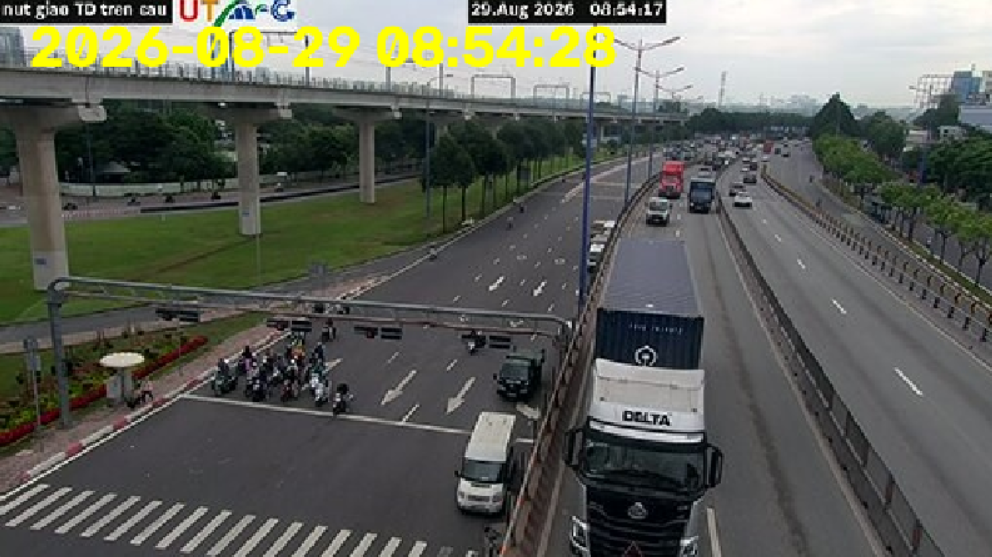
\includegraphics[width=0.85\textwidth]{test_img/1.png}
        \caption{Ảnh thử nghiệm đầu vào \texttt{test\_img/1.png}, ghi nhận các phương tiện ở nhiều khoảng cách và kích thước khác nhau.}
    \end{figure}

    \begin{figure}[htbp]
        \centering
        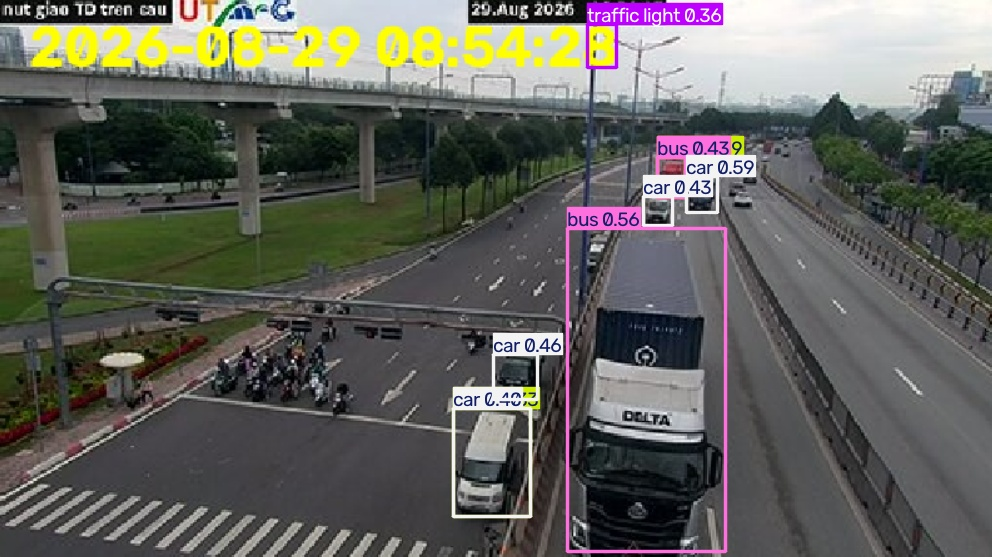
\includegraphics[width=0.85\textwidth]{runs/detect/predict/1.jpg}
        \caption{Kết quả thử nghiệm lưu tại \texttt{runs/detect/predict/1.jpg}. Ảnh hiển thị bounding box, nhãn lớp và độ tin cậy nhận diện.}
    \end{figure}

    Một script thử nghiệm độc lập, \texttt{test\_yolo.py}, khảo sát kích thước lát cắt \texttt{slice\_wh=(512, 512)} và lưu tại \texttt{runs/supervision\_test9.png}. Do đó, không đồng nhất kích thước $512 \times 512$ trong script thử nghiệm với cấu hình lát $256 \times 256$ của luồng vận hành chính thức.

    \subsection{Kiểm tra và tiền xử lý chuỗi thời gian}
    \textbf{Kiểm tra schema:} Pipeline yêu cầu dữ liệu phải có cột \texttt{timestamp} cùng bốn cột đếm phương tiện, \texttt{total} và \texttt{WTI}. \texttt{timestamp} phải hợp lệ, đơn điệu tăng và không trùng lặp; số lượng phương tiện đếm được phải là các số nguyên hữu hạn không âm. Hàm kiểm tra sẽ tính toán lại tổng số xe và chỉ số WTI để phát hiện dữ liệu sai lệch công thức trước khi đưa vào sắp xếp theo thời gian.

    \textbf{Tổng hợp theo phút:} Mỗi khoảng thời gian $[10:00, 10:01)$ được gán mốc nhãn $10:01$, tức thời điểm phút đó đã hoàn tất. Quy ước này giúp ngăn chặn việc sử dụng một phút đang thu thập dở dang như thể đã biết đầy đủ thông tin. Tại mỗi phút hoàn tất, hệ thống tính toán: giá trị trung bình số xe từng loại, trung bình WTI/total, độ lệch chuẩn, giá trị cực đại và số lượng mẫu thu được. Độ lệch chuẩn nội phút sử dụng bậc tự do $\text{ddof} = 0$; những phút chỉ có một mẫu quan sát sẽ có độ lệch chuẩn bằng 0.

    \textbf{Xử lý giá trị thiếu:} Những phút hoàn toàn không thu được mẫu nào được gán giá trị \texttt{NaN} ở các phép đo và số mẫu bằng 0. Pipeline tuyệt đối không tự ý điền giá trị 0 hoặc nội suy để tránh biến khoảng thời gian mất tín hiệu camera thành quan sát giao thông thông thoáng. Hai đầu biên của file CSV không đủ phút sẽ bị loại bỏ. Mọi cửa sổ thời gian bị thiếu lịch sử hoặc thiếu bất kỳ giá trị mục tiêu nào trong 60 phút tiếp theo đều bị loại khỏi tập học có giám sát (supervised dataset).

    \textbf{Chuẩn hóa:} Luồng dự báo không áp dụng các phép biến đổi như \texttt{StandardScaler}, \texttt{MinMaxScaler} hoặc đưa WTI về đoạn $[0, 1]$. Cột \texttt{WTI\_norm} được lưu trong dữ liệu thô theo công thức:
    \[
    \text{WTI\_norm} = \text{WTI} \times [1 + \ln(1 + \text{total})]
    \]
    Mặc dù tên cột chứa tiếp vĩ ngữ ``norm'', công thức này thực chất khuếch đại WTI theo tổng số xe chứ không đưa dữ liệu về khoảng chuẩn. Cả tập đặc trưng lẫn mục tiêu của mô hình hiện tại đều không sử dụng cột này. Việc giữ nguyên WTI ở thang đo gốc giúp sai số MAE và ngưỡng cảnh báo có cùng đơn vị trực quan, dễ đối chiếu.

    \textbf{Chất lượng đầu vào lúc vận hành:} Nhánh mô hình yêu cầu chuỗi 61 phút dữ liệu thực tế liên tục, trong đó mỗi phút phải có ít nhất 3 mẫu hợp lệ. Khi thiếu lịch sử hoặc xuất hiện phút thưa mẫu, hệ thống tự động chuyển sang cơ chế ước lượng tạm thời (nếu có dữ liệu tham chiếu). Khi phút mới nhất hoàn toàn không có mẫu quan sát, hệ thống lập tức dừng đưa ra dự báo.

    \textit{Lưu ý kỹ thuật:} Hàm \texttt{supervised\_data()} trong quá trình huấn luyện và kiểm thử offline chỉ yêu cầu dữ liệu không bị thiếu (\texttt{non-null}), chưa áp dụng đồng loạt điều kiện tối thiểu 3 mẫu/phút như nhánh vận hành thực tế. Vì vậy, tập 956 origin đánh giá offline không đồng nhất hoàn toàn với tập thời điểm mà hệ thống chấp nhận kích hoạt mô hình ngoài thực tế.

    \subsection{Thiết kế 61 đặc trưng}
    Từ chuỗi dữ liệu lịch sử một giờ, hệ thống trích xuất tổng cộng 61 đặc trưng đầu vào cho mô hình:

    \begin{table}[htbp]
        \centering
        \caption{Bảng thiết kế 61 đặc trưng đầu vào}
        \vspace{0.2cm}
        \begin{tabular}{|p{3.2cm}|p{1.5cm}|p{5.5cm}|p{6cm}|}
            \hline
            \textbf{Nhóm đặc trưng} & \textbf{Số lượng} & \textbf{Nội dung chi tiết} & \textbf{Thông tin cung cấp} \\
            \hline
            Phút hiện tại & 11 & Trung bình 4 loại xe; mean, std, max của \texttt{total} và \texttt{WTI}; số mẫu & Mức độ hiện diện, cơ cấu thành phần dòng xe, dao động nội phút và độ phủ dữ liệu. \\
            \hline
            Giá trị trễ (Lags) & 16 & Lag 1, 2, 3, 5, 10, 15, 30, 60 cho cả \texttt{total} và \texttt{WTI} & Nắm bắt trạng thái giao thông gần nhất và mức nền tại các mốc xa hơn trong quá khứ. \\
            \hline
            Thống kê trượt & 26 & Mean (5, 15, 30, 60); std, min, max (5, 15, 30) cho cả \texttt{total} và \texttt{WTI} & Xu hướng trung tâm, biên độ biến thiên và mức độ bất ổn định cục bộ. \\
            \hline
            Độ dốc (Slope) & 6 & Slope 5, 15, 30 cho \texttt{total} và \texttt{WTI} & Hướng tăng/giảm và tốc độ biến thiên trung bình của lưu lượng. \\
            \hline
            Thời gian chu kỳ & 2 & \texttt{hour\_sin}, \texttt{hour\_cos} & Vị trí của thời điểm quan sát trong chu kỳ 24 giờ. \\
            \hline
            \textbf{Tổng cộng} & \textbf{61} & \multicolumn{2}{p{11.5cm}|}{} \\
            \hline
        \end{tabular}
    \end{table}

    Với chuỗi tín hiệu $s$, độ dốc trong mã nguồn được tính bằng công thức hiệu số đơn giản:
    \[
    \text{slope}_w(t) = \frac{s(t) - s(t-w)}{w}
    \]
    Đây không phải là hệ số góc thu được từ phép hồi quy tuyến tính trên toàn bộ cửa sổ $w$. 

    Mã hóa thời gian theo chu kỳ sử dụng hàm $\sin$ và $\cos$:
    \[
    \text{hour\_sin} = \sin\left(\frac{2\pi \times \text{giờ}}{24}\right), \quad \text{hour\_cos} = \cos\left(\frac{2\pi \times \text{giờ}}{24}\right)
    \]
    trong đó giờ là số thực bao gồm cả phần lẻ thập phân tính theo phút. Cách biểu diễn này đảm bảo tính liên tục hình học giữa hai thời điểm ranh giới 23:59 và 00:00.

    Việc khai thác song song cả \texttt{total} và \texttt{WTI} giúp mô hình nắm bắt đồng thời cả mật độ lượng xe lẫn cơ cấu trọng số: hai khung hình có cùng tổng số xe vẫn cho WTI khác biệt rõ rệt khi tỷ lệ xe buýt hoặc xe tải thay đổi. Hàm \texttt{create\_features()} chỉ trích xuất từ dữ liệu hiện tại và quá khứ; hàm \texttt{create\_targets()} dịch chuyển WTI về 60 bước tương lai để tạo nhãn. Cùng một mô-đun được sử dụng đồng bộ cho cả pha huấn luyện lẫn suy luận nhằm loại bỏ rủi ro sai lệch thứ tự cột.

    \subsection{Kiến trúc dự báo và hậu xử lý}
    Hệ thống sử dụng kiến trúc \texttt{MultiOutputRegressor(HistGradientBoostingRegressor)} gồm 60 bộ hồi quy riêng biệt, mỗi bộ phụ trách dự báo cho một bước thời gian (horizon) từ $t+1$ đến $t+60$. Tại thời điểm $t$, tất cả 60 mô hình đều nhận chung vector đầu vào $X(t)$; dự báo tại $t+2$ hoàn toàn không phụ thuộc vào kết quả của $t+1$.

    Thiết kế dự báo trực tiếp (Direct Multi-step) giúp triệt tiêu hoàn toàn hiện tượng tích lũy và khuếch đại sai số qua các bước đệ quy. Ngược lại, do 60 bộ hồi quy học hoàn toàn độc lập, chúng không tự bảo đảm tính liên tục mượt mà của đường cong dự báo theo trục thời gian, đồng thời làm tăng chi phí lưu trữ và suy luận.

    Sau suy luận, chuỗi dự báo được xử lý qua các bước:
    \begin{enumerate}
        \item Chặn dưới giá trị tại 0 ($\max(0, \hat{y})$).
        \item Làm mượt bằng bộ lọc trung bình trượt 3 điểm (Moving Average 3), nối liền với tối đa hai điểm WTI quan sát thực tế gần nhất.
        \item Xác định ETA: Áp dụng quy tắc tìm cửa sổ 5 phút liên tiếp có ít nhất 3 điểm vượt ngưỡng 100 WTI (quy tắc 3/5). Giá trị ETA trỏ đến mốc bắt đầu của cửa sổ đầu tiên thỏa mãn điều kiện.
    \end{enumerate}

    \begin{table}[htbp]
        \centering
        \caption{Các trạng thái hoạt động của hệ thống}
        \vspace{0.2cm}
        \begin{tabular}{|p{4cm}|p{12cm}|}
            \hline
            \textbf{Trạng thái} & \textbf{Ý nghĩa trong hệ thống} \\
            \hline
            \texttt{NORMAL} & Nhánh mô hình không phát hiện cửa sổ vượt ngưỡng nào trong 60 phút tới. \\
            \hline
            \texttt{PROVISIONAL} & Đang hoạt động ở chế độ ước lượng tạm thời và chưa phát hiện nguy cơ vượt ngưỡng. \\
            \hline
            \texttt{WATCH} & Phát hiện cửa sổ dự báo vượt ngưỡng, thời điểm bắt đầu xảy ra sau hơn 5 phút. \\
            \hline
            \texttt{WARNING} & Cửa sổ vượt ngưỡng bắt đầu trong vòng 5 phút tới, hoặc quan sát thực tế đã vượt ổn định. \\
            \hline
            \texttt{INSUFFICIENT\_DATA} & Dữ liệu đầu vào chưa đáp ứng đủ tiêu chuẩn để phát tín hiệu dự báo. \\
            \hline
            \texttt{MODEL\_ERROR} & Xảy ra lỗi trong quá trình suy luận hoặc lỗi cấu trúc dữ liệu bundle. \\
            \hline
        \end{tabular}
    \end{table}

    \subsection{Khởi động và dự báo tạm thời}
    Để giải quyết bài toán khởi động lạnh (Cold-start) khi ứng dụng vừa bật và chưa tích lũy đủ 61 phút quan sát, hệ thống xây dựng một đường tham chiếu gồm 96 ô thời gian (mỗi ô 15 phút) tính từ trung bình của tập \texttt{data1}.

    Hàm \texttt{provisional\_values()} sử dụng tối đa 30 phút thực tế gần nhất để điều chỉnh đường tham chiếu:
    \begin{itemize}
        \item Chênh lệch mức nền giữa thực tế và tham chiếu được dùng để bù trừ mức độ cao/thấp.
        \item Khi có tối thiểu 10 phút dữ liệu thật, hệ thống ước lượng xu hướng biến thiên và chặn hệ số góc trong đoạn $[-1, 1]$ WTI/phút.
        \item Mức độ hiệu chỉnh suy giảm dần theo thời gian qua trọng số hàm mũ $\exp(-h/20)$, và giới hạn độ dốc qua $10 \times [1 - \exp(-h/10)]$, giúp các sai lệch ngắn hạn không bị kéo dài suốt cả giờ.
    \end{itemize}

    Các quan sát tham chiếu được đánh dấu cờ \texttt{is\_reference} và không bao giờ được đưa vào mô hình học máy như dữ liệu thực. Khoảng dữ liệu bị mất trong phiên cũng không bị điền lấp bằng tham chiếu, đảm bảo tính trung thực của phép đo giao thông.

